\documentclass{pnastwo}

%% Packages
\usepackage[T1]{fontenc}
\usepackage[utf8]{inputenc}
\usepackage[english]{babel}
\usepackage{amssymb,amsfonts,amsmath}
\usepackage{graphicx}  %figures
\usepackage{upgreek}
\usepackage{xspace}
%\usepackage{pnastwof}

%% New commands
\newcommand{\micro}{\ensuremath{\upmu}}
\newcommand{\percent}{\%\xspace}
\newcommand{\msub}[1]{\ensuremath{\textnormal{\begin{tiny}#1\end{tiny}}}}
\renewcommand{\d}[1]{\ensuremath{\operatorname{d}\!{#1}}}

%%%%%%%%%%%%%%%%%%%%%%%%%%%%%%
%% Don't type in anything in the following section:
%%%%%%%%%%%%
%% For PNAS Only:
\contributor{Submitted to Proceedings
of the National Academy of Sciences of the United States of America}
\url{www.pnas.org/cgi/doi/10.1073/pnas.0709640104}
\copyrightyear{2008}
\issuedate{Issue Date}
\volume{Volume}
\issuenumber{Issue Number}
%%%%%%%%%%%%
\footlineauthor{ Corresponding author:
    M. Abis, 
    matteo.abis@psi.ch
}

\begin{document}

\title{X-ray phase-contrast imaging at 100 keV on a conventional source}

\author{T.~Thüring%
\affil{1}{Paul Scherrer Institute, 5232 Villigen, Switzerland}%
\affil{2}{Institute for Biomedical Engineering,
    Swiss Federal Institute of Technology,
    Gloriastrasse 35,
8092 Zurich, Switzerland},%
M.~Abis%%
\affil{1}{}%
\affil{2}{},%
Z.~Wang%
\affil{1}{},%
C.~David%
\affil{1}{},%
\and%
M.~Stampanoni%
\affil{1}{}%
\affil{2}{}}

\contributor{Submitted to Proceedings of the National Academy of Sciences
of the United States of America}

%% The \maketitle command is necessary to build the title page.
\maketitle

\begin{article}

\begin{abstract}
    X-ray grating interferometry is a promising imaging technique sensitive
    to attenuation, refraction and scattering of the radiation. Applications
    of this technique in the energy range between 80 and
    150 keV are still largely unexplored due to the
    severe technical challenges. Phase-contrast X-ray imaging at such high
    energies is of relevant scientific and industrial interest, in
    particular for the investigation of materials with high atomic number or
    thickness as well as for medical imaging. Here we show the successful
    implementation of a Talbot-Lau interferometer operated at
    100 keV using a conventional X-ray tube and a
    compact geometry, with a total length of 54 cm. We
    present edge-on illumination of the gratings to overcome their current
    fabrication limits as well as curved structures, to match the beam
    divergence and allow a large field of view on a short and efficient
    setup.
\end{abstract}


%% When adding keywords, separate each term with a straight line: |
\keywords{X-ray phase contrast | grating interferometry | X-ray interferometry}

%% Optional for entering abbreviations, separate the abbreviation from
%% its definition with a comma, separate each pair with a semicolon:
%% for example:
%% \abbreviations{SAM, self-assembled monolayer; OTS,
%% octadecyltrichlorosilane}

\abbreviations{
%acronyms
CT, computed tomography;
SNR, signal-to-noise ratio;
CNR, contrast-to-noise ratio;
SEM, scanning electron microscope;
}
%% ----------------------------------------------------------------------------------------------------------------
%% The first letter of the article should be drop cap: \dropcap{}
%\dropcap{I}n this article we study the evolution of ''almost-sharp'' fronts

\section{Significance statement}

Phase sensitive X-ray imaging techniques provide access to new and
invaluable information compared to traditional absorption-based radiography
and tomography.

Here we show a Talbot-Lau grating interferometer based on a novel optical
design, enabling imaging at X-ray energies of~100 keV and above
with a large field of view as well as a very compact and efficient geometry. 

Our results demonstrate, for the first time, that phase contrast X-ray
imaging can be successfully performed at diagnostically relevant energies
using a conventional X-ray tube, with potential applications spanning from
medical imaging to nondestructive testing or homeland security.

\section{}
\dropcap{X}-ray radiography and CT are standard imaging techniques in
materials and life sciences for the nondestructive examination of samples or
diagnostic tasks in medicine. The underlying contrast mechanism
relies on the different X-ray attenuation properties of different materials
or tissue types. The dominant physical effects contributing to attenuation
are the photoelectric effect and incoherent (Compton) scattering. Besides attenuation, the wave
nature of X-rays reveals another contrast mechanism, which is the phase
shift. The interaction contributing to phase shifts is coherent (Rayleigh)
scattering~\cite{Als-Nielsen2011}.

The attenuation and phase shift properties are described by the complex index of refraction
$n=1-\delta + i \beta$.
The imaginary part $\beta$ is related to the
attenuation coefficient by $\mu = 4 \pi
\beta(\lambda) / \lambda$, while the real part
$\delta(\lambda)$ determines the phase shift 
$\phi = 2 \pi \delta(\lambda) / \lambda$

While the attenuation can be measured with an
X-ray detector as the reduction of the beam intensity, the phase
is not directly observable. Therefore, an optical system is needed to
convert the phase shift into intensity modulations.

Phase-sensitive
imaging is a desirable modality, as it delivers a complementary source of
contrast with respect to absorption by providing direct access 
to the electron density~\cite{Als-Nielsen2011}. Moreover, the combination with
attenuation enables the determination of the effective atomic
number~\cite{Qi2010}.
An enhanced
CNR in images compared to attenuation for certain
materials or tissues~\cite{Pfeiffer2007a,McDonald2009} has also been
demonstrated.

The vast majority of phase-sensitive techniques, including crystal analyzer
based~\cite{Davis1995,Chapman1997} or interferometric~\cite{Bonse1965,Momose1996}
methods rely on X-ray beams of high spatial and temporal coherence, which is
available only at synchrotron sources. Inline
phase contrast~\cite{Snigirev1995,Wilkins1996,Cloetens1996} and
Talbot interferometry~\cite{Cloetens1997,David2002,Momose2003a} need high
spatial coherence but are available on polychromatic microfocus sources.
Phase-contrast imaging using X-ray beams of low temporal \emph{and}
spatial coherence such as conventional low-brilliance X-ray tubes have been
demonstrated with coded
apertures~\cite{Munro2012} and Talbot-Lau
interferometry~\cite{Pfeiffer2006}. Analyzer-based systems have been
recently extended to tube sources~\cite{Nesch2009,Parham2009}
but only at energies up
to the tungsten $K_\alpha$ line at~60 keV.
In addition to phase sensitivity, analyzer-based and Talbot interferometry 
approaches also provide (with different retrieval mechanisms)
information about the integrated local small angle scattering power from
microscopic density fluctuations in a specimen~\cite{Pfeiffer2008}. This signal is known under the name of dark-field, scatter or visibility reduction contrast.

High-energy Talbot interferometry has been reported so far using a
synchrotron source at nominal energies of
82 keV~\cite{Willner2013}.
Using a low-brilliance X-ray tube, Talbot-Lau interferometry was
applied so far at 60 keV mean energy~\cite{Donath2009}.
Medical imaging applications may benefit from phase contrast at higher
energies: chest or abdominal
radiography or CT require an acceleration voltage between 100 and
150 kVpeak. Other potential applications are homeland
security or chip failure analysis, which require high energies for the
visualization of materials of high density and atomic number.

Here we introduce a method for phase contrast imaging which works on
conventional X-ray sources, covers the entire diagnostic X-ray energy range
and is compatible with compact imaging arrangements. The approach is based
on
Talbot-Lau
interferometry~\cite{Pfeiffer2006} and employs an edge-on illumination approach for the grating design and
arrangement. 
Our solution removes one on the major hurdle which prevented grating interferometry to be applied at very high X-ray energies so far, namely the fabrication of gratings with high-aspect ratios.
 The aspect
ratio, given by
\begin{equation}
    \text{R} = \frac{2h}{p},
\end{equation}
where $p$ is the grating period and $h$ the  structure
height, is normally limited by the fabrication process, usually
photolithography~\cite{David2002} or X-ray lithography~\cite{Mohr2012} as grating
structures tend to collapse or deform (e.g. due to capillary forces) if
the aspect ratio is too high. For a given setup length these parameters
depend on the target energy $E$ according to $p \propto
1/\sqrt{E}$ and $h \propto E^3$, and therefore $\textnormal{R}
\propto E^{7/2}$~\cite{Momose2003a}. If at $E=25 keV$ an aspect ratio
for the absorption grating around $\textnormal{R}=30$ is necessary for a
reasonable length of the experimental arrangement, it would have to be at
least $128$ for $E=100 keV$. Moreover, when using a
broad spectrum, photons above the design energy should also be
efficiently blocked by the gratings, which requires even higher aspect ratios.
The largest aspect ratios achieved by current fabrication techniques~\cite{David2007,Kenntner2010} are around 60.

Our design introduces the edge-on
illuminated,  circularly aligned structures. Edge-on illumination
(Fig.~\ref{Fig:schematic}), as
opposed to face-on illumination, exploits the dimension along the grating
lines to form a high aspect ratio of the structures in the direction of the beam. The
effective structure height of the grating is then determined by the grating
dimension along the grating lines, which essentially allows arbitrarily high
aspect ratios. 

Increasing the aspect ratio of the gratings typically leads to a
reduction of the field of view due to the change of the grating transmission
function at high incident angles. In order to overcome this problem, the grating lines are circularly aligned 
with a radius equal to the distance to the source. 
This allows to achieve an arbitrarily large field of view in a fan-beam
geometry, a significant improvement compared to face-on based and glancing
angle~\cite{Stutman2012a} approaches.

The combination of edge-on illumination and circularly aligned structures
enables phase-contrast imaging at arbitrary design energies and with a
maximum field of view in the horizontal direction ($x$ direction). These
advantages come at the expense of a limited field of view in the vertical
direction ($y$ direction), which is, depending on the X-ray detector,
typically a few pixels. 
However, radiographic 2D imaging can be obtained by scanning the sample or a thin fan
beam. The scanning technique has been demonstrated to deliver less dose than
the conventional approach based on the illumination of a large area. In
digital mammography, for instance, where dose is a critical issue, Philips'
MicroDose system combines a scanning approach with an highly collimated fan
beam~\cite{Aslund2007}. Thanks to the high collimation, the dose deposited
on  patients has been reported to be significantly lower than with other
instruments based on the illumination of a large area
detector~\cite{Oduko2010}.
Similarly, for tomographic images,
the approach allows single slice CT or full 3D imaging in scanning mode.

Grating design and fabrication is nonstandard and involves a complex mask
design, as shown in Fig.~\ref{Fig:grating_mask}. Multiple gratings can reside on a
silicon chip with their specific structure length and curvature. For the
current experiments, a symmetric interferometer with a grating period of $p
= 2.8 \micro m$ for all gratings has been used. The design energy
is 100 keV and the beam splitter grating periodically
shifts the phase by zero and $\pi$ at this energy~\cite{David2002}. Using
gold as the phase shifting material, a structure length of
$h_1 = 19.8 \micro m$ is required. The analyzer grating is an absorption mask
for sensing slight changes of the interference pattern generated by the beam
splitter~\cite{Momose2003a}. With a structure length of $h_2 =
800 \micro m$
it can sufficiently attenuate X-rays up to energies of 
160 keV. Beam splitter and analyzer grating are
separated at the first fractional Talbot order~\cite{Weitkamp2005},
resulting in an intergrating distance of 158 mm. The
source grating splits the relatively large focal spot ($\sim
1 mm$) into an array of individually coherent, but mutually
incoherent sources~\cite{Pfeiffer2006}. It is also made of gold structures
with a length of $h_0 = h_2 = 800 \micro m$.

Due to the high spectral acceptance~\cite{Weitkamp2005,Thuering2013c} of the
interferometer (50 keV to
more than 160 keV) and the high attenuation efficiencies of
the source and analyzer gratings ($>90\%$ up to
160 keV), the voltage of the X-ray source was set to
the maximum of 160 kV. With a grating structure height of
approximately 100 \micro m, the field of view in the vertical
direction is limited to one detector pixel row. In the horizontal direction,
the field of view is only limited by the grating size to
30 mm, but wider gratings can be fabricated with this
method and the available technology on larger wafers. In addition to the standard components (source,
camera, interferometer), two optical slits, one in front of the source
grating, the other in front of the camera, were required for the collimation
of the beam in the vertical direction. 

\section{Results and discussion}
Fig.~\ref{Fig:img_chip} shows a radiographic scan of an electronic chip.
Several resistors and an integrated circuits are located on different layers
on the chip. The images were acquired in scanning mode, using a step size of
100 \micro m along the $y$ axis. For a better comparison of the
magnified phase and attenuation images, the attenuation image has been
replaced with the differential attenuation image, which was obtained by
digital differentiation. In the attenuation image, the contrast of the soldering points of
the integrated circuit is reduced underneath the resistors, while in
the phase image, they can clearly be identified. The reduced contrast of the 
soldering points in the absorption image is due to beam hardening. The spectrum
impinging on these soldering point is hardened by the resistors in the upper
layer, resulting in lower absorption contrast. Due to the weaker energy
dependency of phase shifts ($1/E$ compared to $1/E^3$), phase-contrast images
are less sensitive to beam hardening~\cite{Chabior2011a}, which explains the
lower contrast reduction of the soldering points underneath the resistors in the
phase image of the chip. This result shows the benefit of the phase contrast in
high-energy X-ray imaging, which may be useful to identify flaws in multilayered
structures such as electronic chips.

Edge-on illuminated grating interferometry finally allows phase contrast
imaging to be performed at high energies ($>100 keV$) on conventional X-ray
sources. With a circular distribution of the gratings, the diffracting and
absorbing structures can be matched to the divergent beam, even for very
compact geometries. Short, high-energy phase-contrast systems enable the
efficient investigation of high-density materials or thick samples,
adding information on electron density and integrated small angle scattering
power to the conventional absorption based signal. This will improve
material discrimination and density sensitivity capabilities in future
X-rays or even neutron~\cite{Grunzweig2008} investigations.

%% == end of paper:

%% Optional Materials and Methods Section
%% The Materials and Methods section header will be added automatically.

%% Enter any subheads and the Materials and Methods text below.
\begin{materials}
Edge-on illuminated gratings were manufactured by Microworks GmbH, Germany, using a LIGA process~\cite{Kenntner2010}. Each grating
resides on a $5 \times 60 mm^2$ silicon chip and several
grating chips are fabricated on a single 4 inch silicon wafer. The
experimental arrangement for a design energy at 100 keV
is a symmetric Talbot-Lau interferometer with a grating period of $p =
2.8 \micro m$ for all gratings. The distance from the source
grating to the analyzer grating is 32 cm and the source
grating is positioned 23 cm away from the source.

The X-ray source is a COMET MXR-160HP/11 X-ray tube with a maximum output
voltage of 160 kV. In the experiment, it was set to the
maximum voltage. The focal spot size is approximately
1 mm. The detector is a CCD camera from Finger Lakes
Instruments. A cesium iodide (CsI:Ti) scintillator of 600 \micro m
thickness converts the X-rays to visible light and is coupled with
an optical lens projecting the image onto the CCD. The effective pixel size
is 80 \micro m. The collimating slit right after the source is 
25 \micro m large, while the second slit before the detector is
100 \micro m.

In Fig.~\ref{Fig:img_chip}, image acquisition involved 24 phase steps per
line and an exposure time of 15 seconds per step. The long
exposure times are mostly constrained by the low average visibility of the
gratings (5 \percent). The exposure time was chosen in order to
get a low noise in the differential phase image. The SNR is
proportional to the visibility and the square root of the exposure
time~\cite{Raupach2011}.
This implies that the exposure times can easily drop by an order of
magnitude as these gratings become comparable in quality to those developed
in the last ten years. 
Smaller regions of these gratings actually exhibit a visibility up
to~14 \percent already, indicating that this goal is reachable as the
fabrication becomes more reliable and uniform.
\end{materials}


%% Optional Appendix or Appendices
%% \appendix Appendix text...
%% or, for appendix with title, use square brackets:
%% \appendix[Appendix Title]

\begin{acknowledgments}
We thank Gordan Mikuljan, Peter Modregger and István Mohácsi from the Paul
Scherrer Institute (PSI), Switzerland, for the
work on the mechanical design, the scientific advice, and the SEM images
respectively, Joachim Schulz and Marco Walter from
Microworks GmbH, Germany, for the competent support on grating design
issues, Christian Kottler and Vincent Revol from Centre Suisse
d'Electronique et de Microtechnique (CSEM), Switzerland for the fruitful
discussions on the design of the system. This work has been partially
supported by the Competence Centre for Materials Science and Technology
(CCMX) of the ETH Board, Project Nr. 61 and by the ERC Grant ERC-2012-StG 310005-PhaseX.
\end{acknowledgments}

%% PNAS does not support submission of supporting .tex files such as BibTeX.
%% Instead all references must be included in the article .tex document. 
%% If you currently use BibTeX, your bibliography is formed because the 
%% command \verb+\bibliography{}+ brings the <filename>.bbl file into your
%% .tex document. To conform to PNAS requirements, copy the reference listings
%% from your .bbl file and add them to the article .tex file, using the
%% bibliography environment described above.  

%%  Contact pnas@nas.edu if you need assistance with your
%%  bibliography.

% Sample bibliography item in PNAS format:
%% \bibitem{in-text reference} comma-separated author names up to 5,
%% for more than 5 authors use first author last name et al. (year published)
%% article title  {\it Journal Name} volume #: start page-end page.
%% ie,
% \bibitem{Neuhaus} Neuhaus J-M, Sitcher L, Meins F, Jr, Boller T (1991) 
% A short C-terminal sequence is necessary and sufficient for the
% targeting of chitinases to the plant vacuole. 
% {\it Proc Natl Acad Sci USA} 88:10362-10366.

%\bibliographystyle{pnas}
%\bibliography{library}
\begin{thebibliography}{10}

\bibitem{Als-Nielsen2011}
Als-Nielsen J, McMorrow D (2011) {\em {Elements of modern X-ray physics}}.

\bibitem{Qi2010}
Qi Z, Zambelli J, Bevins N, Chen GH (2010) {Quantitative imaging of electron
  density and effective atomic number using phase contrast CT.}
\newblock {\em Physics in medicine and biology} 55:2669--77.

\bibitem{Pfeiffer2007a}
Pfeiffer F et~al. (2007) {High-resolution brain tumor visualization using
  three-dimensional x-ray phase contrast tomography.}
\newblock {\em Physics in medicine and biology} 52:6923--6930.

\bibitem{McDonald2009}
McDonald SA et~al. (2009) {Advanced phase-contrast imaging using a grating
  interferometer}.
\newblock {\em Journal of Synchrotron Radiation} 16:562--572.

\bibitem{Davis1995}
Davis T, Gao D, Gureyev T, Stevenson A, Wilkins S (1995) {Phase-contrast
  imaging of weakly absorbing materials using hard X-rays}.
\newblock {\em Nature} 373:595--598.

\bibitem{Chapman1997}
Chapman D et~al. (1997) {Diffraction enhanced x-ray imaging}.
\newblock {\em Physics in Medicine and Biology} 42:2015--2025.

\bibitem{Bonse1965}
Bonse U, Hart M (1965) {An x-ray interferometer}.
\newblock {\em Applied Physics Letters} 6:155--156.

\bibitem{Momose1996}
Momose A, Takeda T, Itai Y, Hirano K (1996) {Phase-contrast X-ray computed
  tomography for observing biological soft tissues}.
\newblock {\em Nature Medicine} 2:473--475.

\bibitem{Snigirev1995}
Snigirev A, Snigireva I, Kohn V, Kuznetsov S, Schelokov I (1995) {On the
  possibilities of x-ray phase contrast microimaging by coherent high-energy
  synchrotron radiation}.
\newblock {\em Review of Scientific Instruments} 66:5486--5492.

\bibitem{Wilkins1996}
Wilkins S, Gureyev T, Gao D, Pogany A, Stevenson A (1996) {Phase-contrast
  imaging using polychromatic hard X-rays}.
\newblock {\em Nature} 384:335--338.

\bibitem{Cloetens1996}
Cloetens P, Barrett R, Baruchel J, Guigay J, Schlenker M (1996) {Phase objects
  in synchrotron radiation hard x-ray imaging}.
\newblock {\em Journal of Physics D: Applied Physics} 29:133--146.

\bibitem{Cloetens1997}
Cloetens P, Guigay J, {De Martino} C, Baruchel J, Schlenker M (1997)
  {Fractional Talbot imaging of phase gratings with hard x rays.}
\newblock {\em Optics letters} 22:1059--61.

\bibitem{David2002}
David C, N\"{o}hammer B, Solak H, Ziegler E (2002) {Differential x-ray phase
  contrast imaging using a shearing interferometer}.
\newblock {\em Applied Physics Letters} 81:3287--3289.

\bibitem{Momose2003a}
Momose A et~al. (2003) {Demonstration of X-Ray Talbot Interferometry}.
\newblock {\em Japanese Journal of Applied Physics} 42:L866--L868.

\bibitem{Munro2012}
Munro P, Ignatyev K, Speller R, Olivo A (2012) {Phase and absorption retrieval
  using incoherent X-ray sources}.
\newblock {\em Proceedings of the National Academy of Sciences} 2012:2--7.

\bibitem{Pfeiffer2006}
Pfeiffer F, Weitkamp T, Bunk O, David C (2006) {Phase retrieval and
  differential phase-contrast imaging with low-brilliance X-ray sources}.
\newblock {\em Nature Physics} 2:258--261.

\bibitem{Nesch2009}
Nesch I et~al. (2009) {The design and application of an in-laboratory
  diffraction-enhanced x-ray imaging instrument.}
\newblock {\em The Review of scientific instruments} 80:093702.

\bibitem{Parham2009}
Parham C, Zhong Z, Connor DM, Chapman LD, Pisano ED (2009) {Design and
  Implementation of a Compact Low-Dose Diffraction Enhanced Medical Imaging
  System}.

\bibitem{Pfeiffer2008}
Pfeiffer F et~al. (2008) {Hard-X-ray dark-field imaging using a grating
  interferometer}.
\newblock {\em Nature Materials} 7:134--137.

\bibitem{Willner2013}
Willner M et~al. (2013) {Quantitative X-ray phase-contrast computed tomography
  at 82 keV}.
\newblock {\em Optics express} 21:4155--4166.

\bibitem{Donath2009}
Donath T et~al. (2009) {Inverse geometry for grating-based x-ray phase-contrast
  imaging}.
\newblock {\em Journal of Applied Physics} 106:054703.

\bibitem{Mohr2012}
Mohr J et~al. (2012) {High aspect ratio gratings for X-ray phase contrast
  imaging}.
\newblock 41:41--50.

\bibitem{David2007}
David C et~al. (2007) {Fabrication of diffraction gratings for hard X-ray phase
  contrast imaging}.
\newblock {\em Microelectronic Engineering} 84:1172--1177.

\bibitem{Kenntner2010}
Kenntner J et~al. (2010) {\em {Front- and backside structuring of gratings for
  phase contrast imaging with x-ray tubes}}.
\newblock Vol.{} 7804, p. 780408.

\bibitem{Stutman2012a}
Stutman D, Finkenthal M (2012) {Glancing angle Talbot-Lau grating
  interferometers for phase contrast imaging at high x-ray energy}.
\newblock {\em Applied physics letters} 101:91108.

\bibitem{Aslund2007}
{\AA slund, M} (2007) Ph.D. thesis.

\bibitem{Oduko2010}
Oduko JM, Young KC, Burch A (2010) in {\em Digital Mammography}, Lecture Notes
  in Computer Science, eds.{} Martí J, Oliver A, Freixenet J, Martí R.
\newblock (Springer Berlin Heidelberg) Vol.{} 6136, pp. 365--370.

\bibitem{Weitkamp2005}
Weitkamp T et~al. (2005) {X-ray phase imaging with a grating interferometer}.
\newblock {\em Optics Express} 13:6296--6304.

\bibitem{Thuering2013c}
Thuering T et~al. (2013) {Energy resolved X-ray grating interferometry}.
\newblock {\em Applied Physics Letters} 102:191113.

\bibitem{Chabior2011a}
Chabior M et~al. (2011) {Beam hardening effects in grating-based x-ray
  phase-contrast imaging}.
\newblock {\em Medical Physics} 38:1189.

\bibitem{Grunzweig2008}
Gr\"{u}nzweig C et~al. (2008) {Design, fabrication, and characterization of
  diffraction gratings for neutron phase contrast imaging.}
\newblock {\em The Review of scientific instruments} 79:053703.

\bibitem{Raupach2011}
Raupach R, Flohr TG (2011) {Analytical evaluation of the signal and noise
  propagation in x-ray differential phase-contrast computed tomography.}
\newblock {\em Physics in medicine and biology} 56:2219--2244.

\end{thebibliography}

\end{article}
%%%%%%%%%%%%%%%%%%%%%%%%%%%%%%%%%%%%%%%%%%%%%%%%%%%%%%%%%%%%%%%%

%% Adding Figure and Table References
%% Be sure to add figures and tables after \end{article}
%% and before \end{document}

%% For figures, put the caption below the illustration.
%%
%% \begin{figure}
%% \caption{Almost Sharp Front}\label{afoto}
%% \end{figure}

%% For Tables, put caption above table
%%
%% Table caption should start with a capital letter, continue with lower case
%% and not have a period at the end
%% Using @{\vrule height ?? depth ?? width0pt} in the tabular preamble will
%% keep that much space between every line in the table.

%% \begin{table}
%% \caption{Repeat length of longer allele by age of onset class}
%% \begin{tabular}{@{\vrule height 10.5pt depth4pt  width0pt}lrcccc}
%% table text
%% \end{tabular}
%% \end{table}

%% For two column figures and tables, use the following:

%% \begin{figure*}
%% \caption{Almost Sharp Front}\label{afoto}
%% \end{figure*}

%% \begin{table*}
%% \caption{Repeat length of longer allele by age of onset class}
%% \begin{tabular}{ccc}
%% table text
%% \end{tabular}
%% \end{table*}

\begin{figure}
    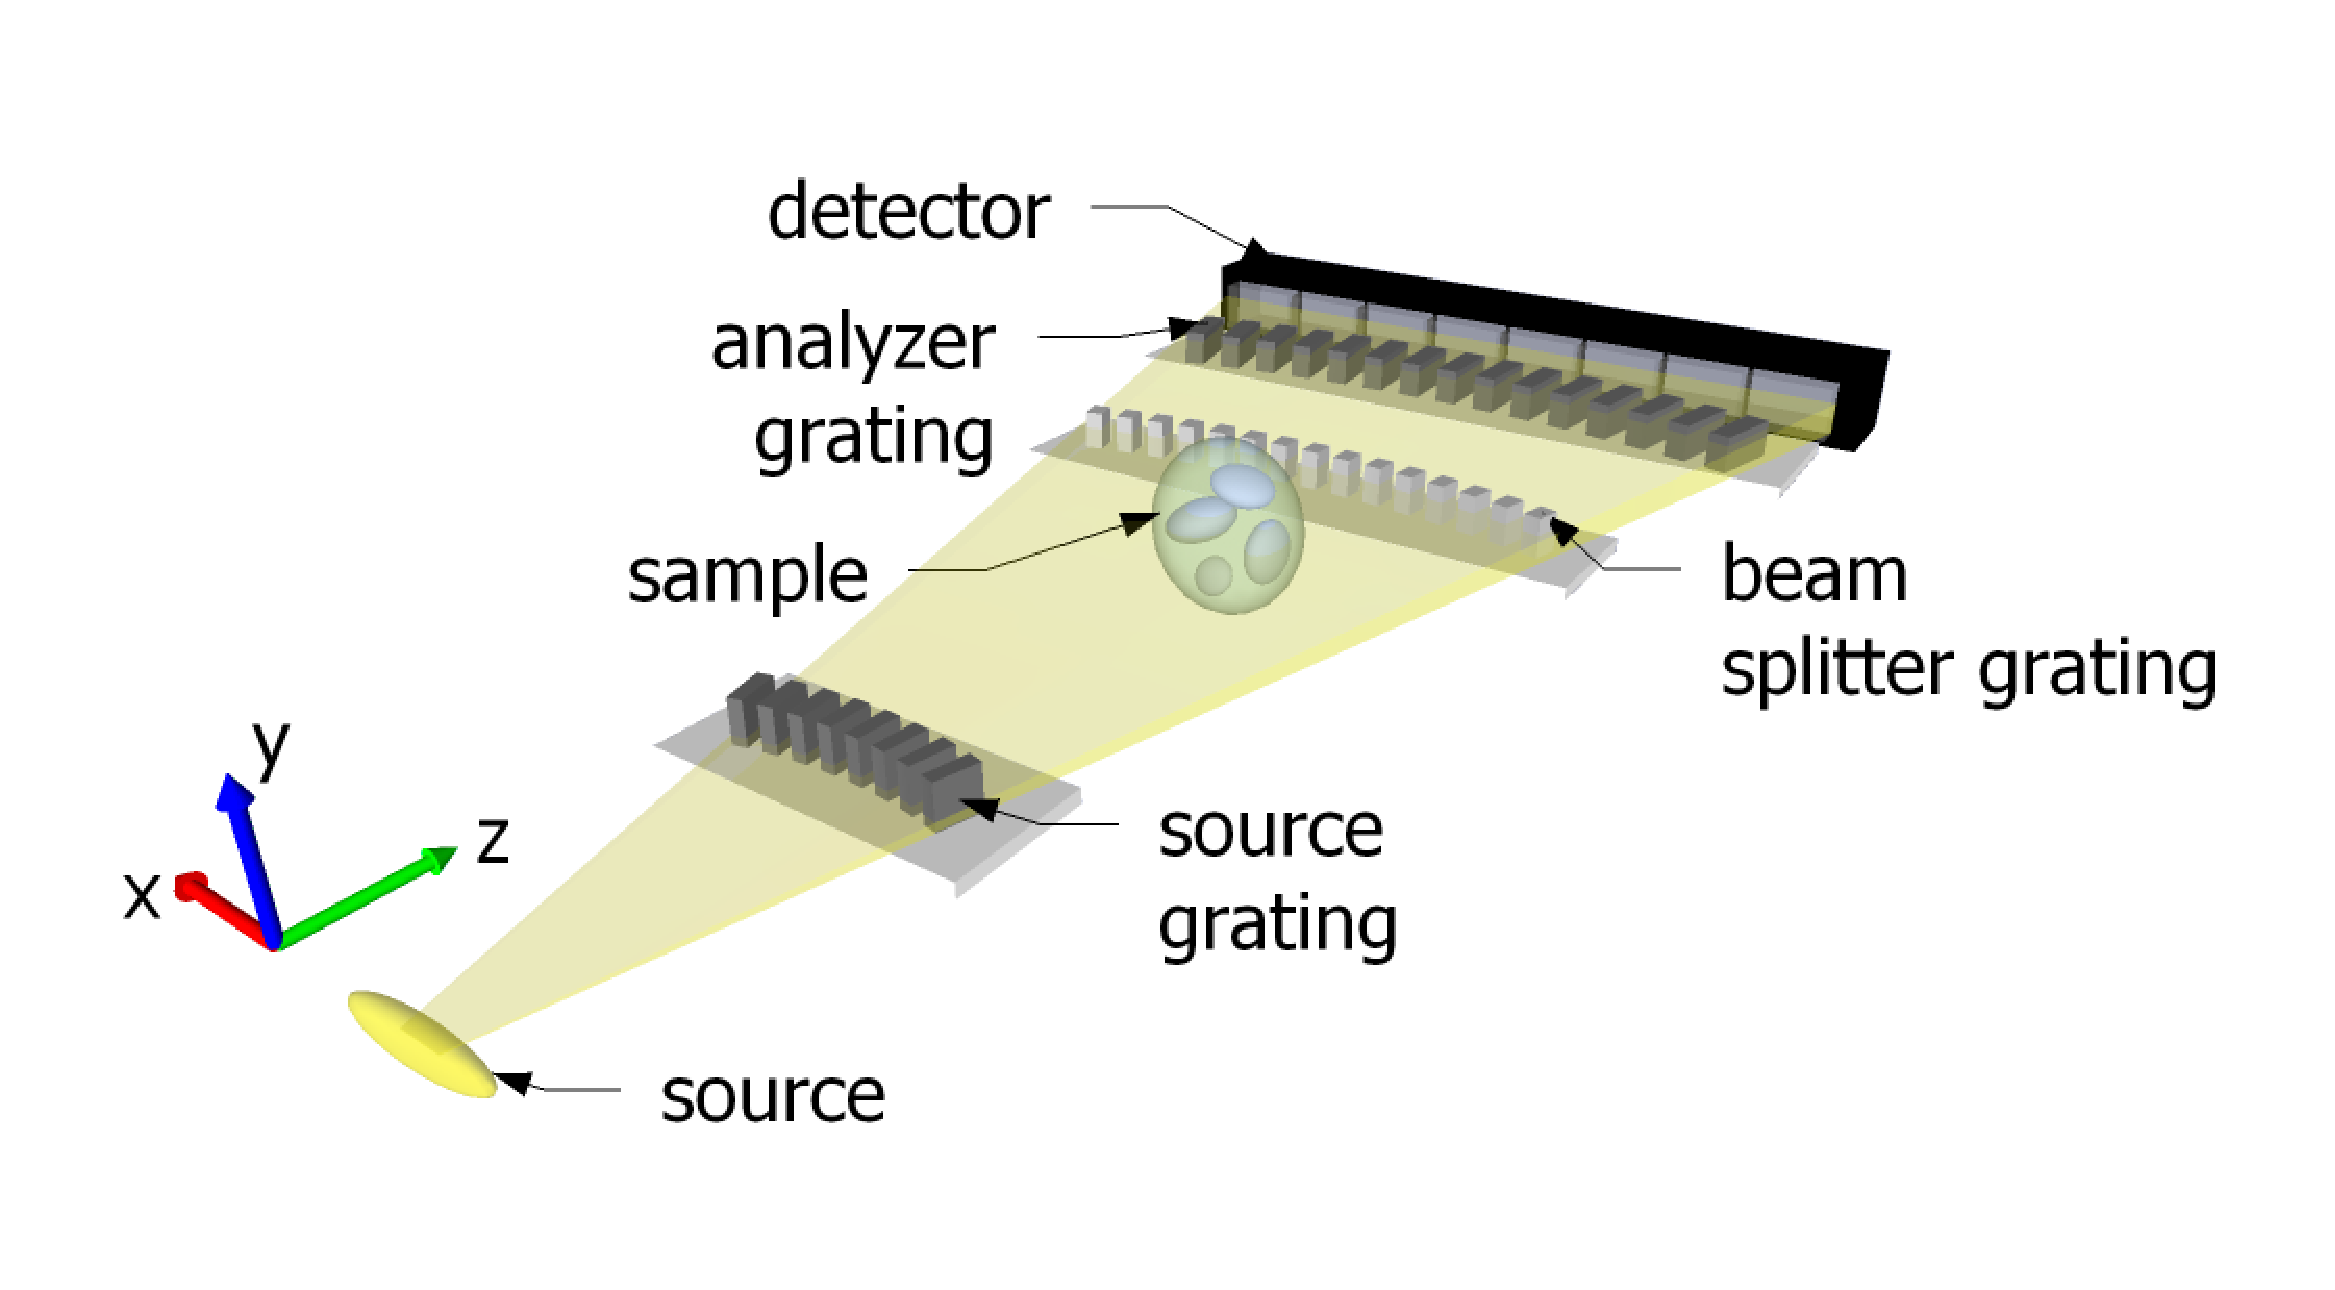
\includegraphics[width=.5\textwidth]{figures/figure1.eps}
    \caption{Schematic of a grating
        interferometer for X-ray energies between 60 and
        150 keV in edge-on illumination mode. The
        aspect ratio is defined by the ratio of the travelling distance along the
        grating lines and the period and can be arbitrarily long. In order to maximise
        the field of view, the grating structures are aligned on an
    arc.}
    \label{Fig:schematic}
\end{figure}

\begin{figure}
    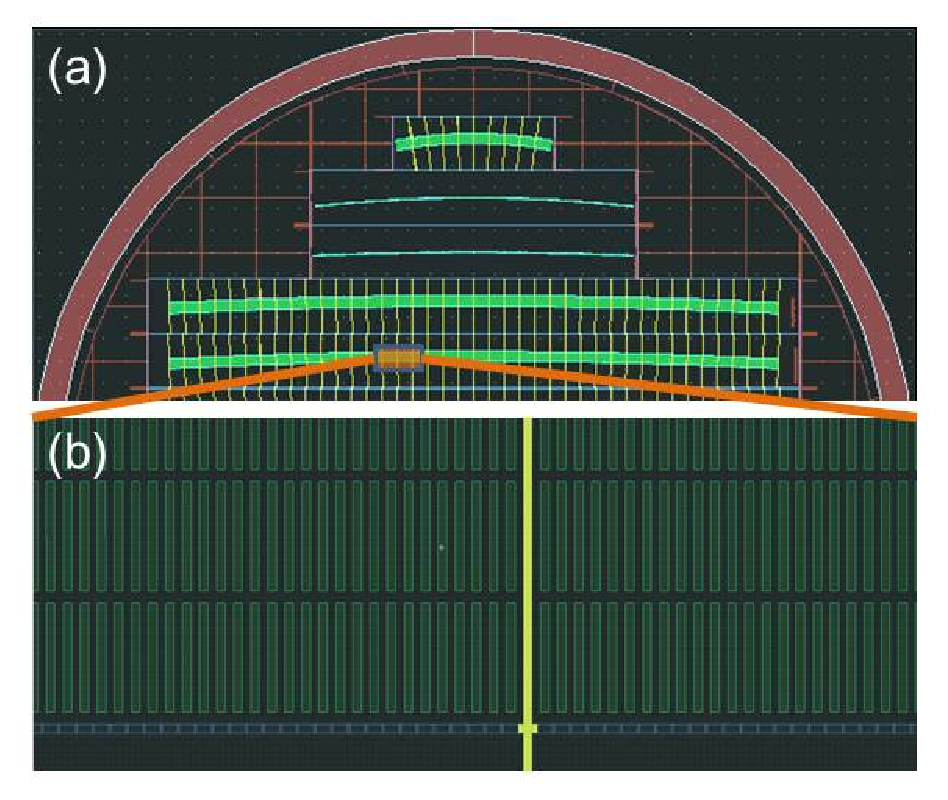
\includegraphics[width=.5\textwidth]{figures/grating_mask.eps}
    \caption{Grating design mask for
        the edge-on illumination approach and SEM
        image of the grating. The top part of the 4 inch wafer shows
        five grating chips. The
        gratings have different curvatures which are specific to the grating
        interferometer geometry. 
        The SEM image shows the gold structures and the interrupting bridges
        that prevent the lamellae from collapsing~\cite{Kenntner2010}.}
        \label{Fig:grating_mask}
\end{figure}

\begin{figure}
    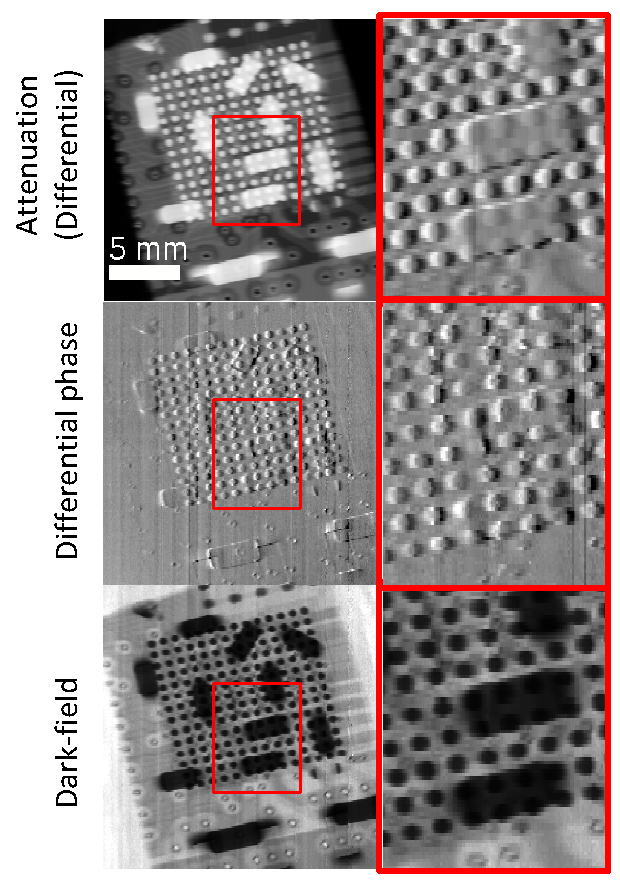
\includegraphics[width=.5\textwidth]{figures/img_chip_dabs.eps}
    \caption{Radiographic scan of an electronic chip. The image was acquired
        with 24 phase steps per line and an exposure time of 15 s per
    step. The top right image shows the differential absorption image.}
    \label{Fig:img_chip}
\end{figure}

\end{document}
